\chapter{Data Analysis}
\label{chap:ana}

General overview: maximum-likelihood fit (introduce NLL), error correction for background,
simultaneous in KK-mass bins and tagging categories

\section{Decay-Candidate Selection and Background}
\label{sec:ana_bkgSub}
show mass-fit results in $\cthetal$ bins
\begin{figure}[htb]
  \centering
  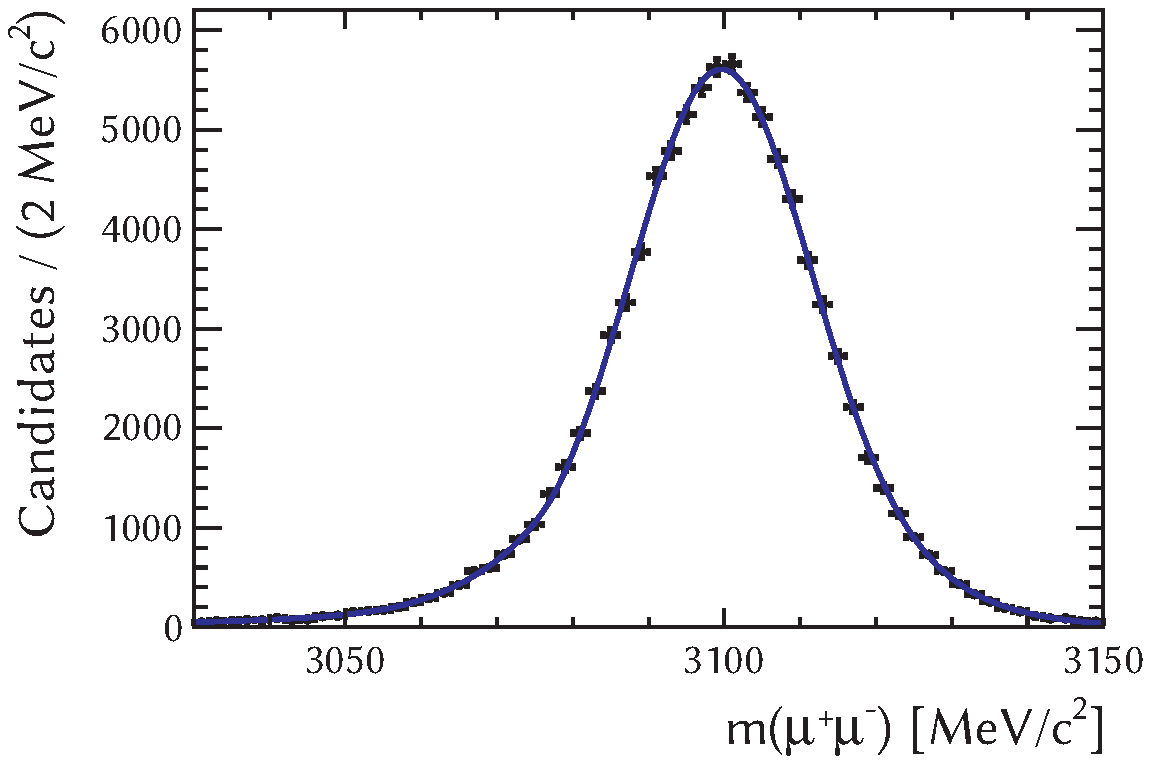
\includegraphics[width=0.7\textwidth]{graphics/analysis/mumuMass}
  \caption{Background-subtracted distribution of \BstoJpsiKK{} decays in $\mumu$ mass.}
  \label{fig:mumuMass}
\end{figure}
\begin{figure}[htb]
  \centering
  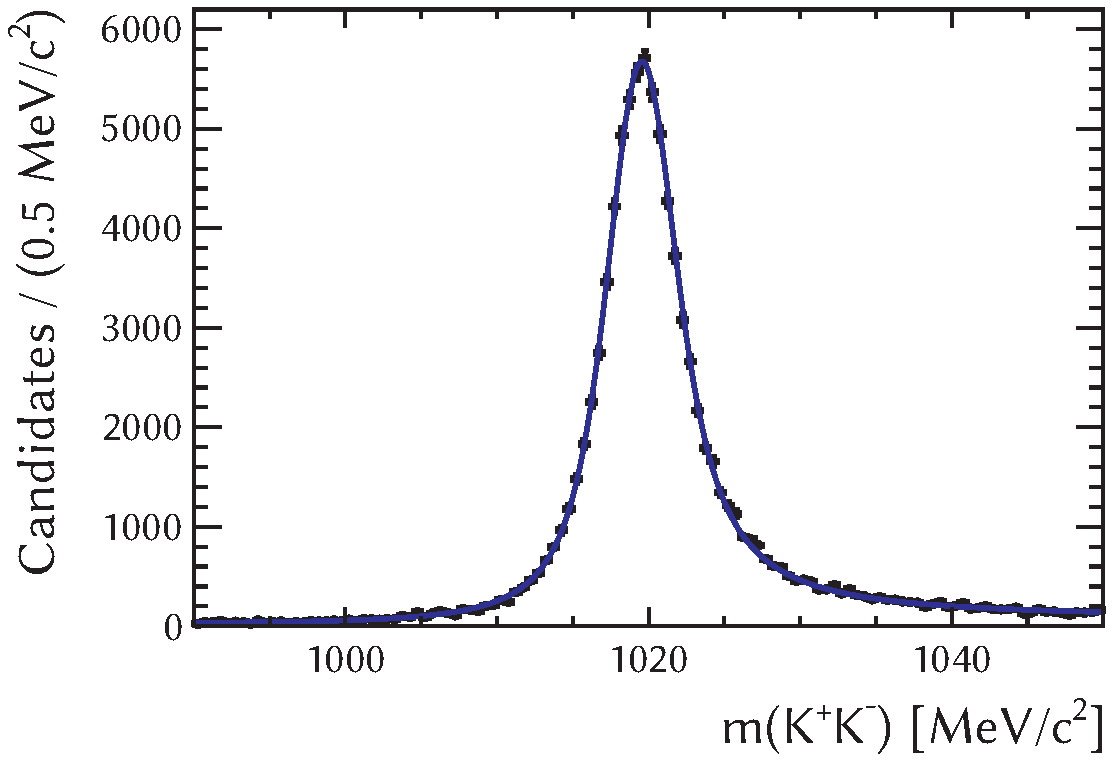
\includegraphics[width=0.7\textwidth]{graphics/analysis/KKMass}
  \caption{Background-subtracted distribution of \BstoJpsiKK{} decays in $\KK$ mass.}
  \label{fig:KKMass}
\end{figure}

\section{Decay Time}
\label{sec:ana_time}
mention reconstruction-acceptance model (linear/exponential/quadratic in time)

\subsection{Resolution}
\label{subsec:ana_time_res}
mention how to handle conditional observables for plots and toys

\subsection{Acceptance}
\label{subsec:ana_time_acc}

\section{Decay Angles}
\label{sec:ana_angles}

\section{\texorpdfstring{$\KK$}{KK}-Mass Integrals}
\label{sec:ana_KKIntegrals}

Discuss trend in phases.
Nominal: $\phimes$ parameterized with a relativistic Breit-Wigner shape, $\fzero$ with a Flatt\'e shape, resolution from MC.
\begin{table}[h]
  \centering
  \caption{S-wave--$\Jpsiphi$ coupling factors in the six $\KK$-mass bins ($\CSP^i$).}
  \label{tab:CSPFactors}
  \begin{tabular}{cccc}
    bin     & nominal  &  +20\% resolution  &  uniform S-wave  \\
    \hline
    1       & 0.9178   &  0.9152            &  0.9586          \\
    2       & 0.9022   &  0.8797            &  0.9110          \\
    3       & 0.8619   &  0.8357            &  0.8618          \\
    4       & 0.8875   &  0.8599            &  0.8828          \\
    5       & 0.9360   &  0.9207            &  0.9227          \\
    6       & 0.9641   &  0.9624            &  0.9110          \\
  \end{tabular}
\end{table}

\section{Flavour Tagging}
\label{sec:ana_tagging}
mention how to handle conditional observables for plots and toys,
explain why nuisance asymmetries can be ignored

\begin{equation}
  \begin{aligned}
    \label{eq:diffRateObs}
    \left(\frac{\ud^{4} \Gamma}{\ud t \;\ud\Omega}\right)_{\qf,\,i}^{\text{obs}}\
      &\propto\ (1-\wTag[\qf,\,i]) \left(\avgCEven[i] + \qf\,\avgCOdd\right)\left(\even + \qf\,\odd\right) \\
      &\qquad\quad+ \wTag[-\qf,\,i] \left(\avgCEven[i] - \qf\,\avgCOdd\right)\left(\even - \qf\,\odd\right) \\
    &\propto\ \left[\avgCEven[i] + \qf\,\dil[i]\left(\avgCOdd[i] - \ADilWTag[i]\,\avgCEven[i]\right)\right]\even \\
      &\qquad\quad+ \left[\avgCOdd[i] + \qf\,\dil[i]\left(\avgCEven[i] - \ADilWTag[i]\,\avgCOdd[i]\right)\right]\odd
  \end{aligned}
\end{equation}


\section{Simulation}
\label{sec:ana_sim}
discuss both detector simulation (with correction for kinematic distributions) and toys
